% This example An LaTeX document showing how to use the l3proj class to
% write your report. Use pdflatex and bibtex to process the file, creating 
% a PDF file as output (there is no need to use dvips when using pdflatex).

% Modified 

\documentclass{l3proj}
\usepackage[toc]{glossaries}
\usepackage[toc,page]{appendix}
\usepackage{multicol}
\usepackage{listings}
\usepackage{color}
\makeglossaries
\begin{document}

%%%%%%%%%%%%%%%%%%%%

%% IMPORTANT
% the glossary does not display in writelatex.com, but if you download as zip from the projects tab and run the makefile from the repo on github it should be displayed correctly (it won't let me have the makefile on here!)

%% also it doesn't work in the lab as the glossary package is not installed in order to compile

%%GLOSSARY ENTRIES
%for help see link http://mirrors.ibiblio.org/CTAN/macros/latex/contrib/glossaries/glossariesbegin.pdf



\newglossaryentry{middleware}{name=middleware,description={Middleware sits between the hardware and software of a system}}
\newglossaryentry{stack}{name=stack, description={provides software that is easily reusable}}
\newglossaryentry{ubuntu}{name=Ubuntu, description={is a Linux Operating System on which \acrshort{ros} is dependant}}
\newglossaryentry{opencv}{name=OpenCV, description={is a library of programming functions mainly aimed at real-time computer vision, developed by Intel}}
\newglossaryentry{asus}{name=Asus, description={is a multinational computer hardware and electronics company}}
\newglossaryentry{europroj}{name=EU-FP7, description={Europen Union Funded project for research and technology}}
\newglossaryentry{xtion}{name=Xtion, description={A camera made by company ASUS, similar to Microsoft's X-Box Kinect}}
\newglossaryentry{pymatbridge}{name=pymatbridge, description={a set of python and matlab functions with the goal of providing an easy, seamless way to call Matlab functions within Python}}

\newglossaryentry{matlab}{name=MATLAB, description={(matrix laboratory) is a numerical computing environment and fourth-generation programming language}}
\newglossaryentry{potrace}{name=Potrace, description={is an open-source, cross-platform computer program which converts bitmapped images into vector graphics}}
\newacronym{clopema}{CLoPeMa}{Clothes Perception and Manipulation}
\newacronym{ros}{ROS}{Robot Operating System}

\title{Creating an exciting demonstration for the CloPeMa robot}
\author{Michael Cromie -- 1003492 \\
		Fraser Leishman -- 1102103 \\
        Edvin Malinovskis -- 2039411 \\
        Andrew McDonald -- 1102115  \\
        Matthew Paterson -- 1102374 \\
        }
\date{\today}
\maketitle
\begin{abstract}
In this dissertation we will show our approach in trying to create an interesting and exciting demonstration in showing off the capabilites of a state-of-the-art robot that specialises in the folding of garments. Our goals were achieved through the use of a software framework that is used to develop robots and also open source vision software.
\end{abstract}
\educationalconsent
\tableofcontents
%==============================================================================
\chapter{Introduction}
\label{intro}
\section{Project Synopsis}
The aim of the project was to implement a drawing robot which would: capture an image of a participant's face; detect the lines of the image using software; guide the robots arm to grasp a marker pen then to move corresponding to the instructions built from the line detected image. 

\section{Background}
\subsection{Robot}
The \acrshort{clopema} robot is a purpose built robot designed for the manipulation of garments that surround it. This 750Kg robot consists of the base that it sits upon and also two arms that can pivot and rotate to maximise the dexterity of the robot. The base is able to rotate \begin{math} 270\,^{\circ}
\end{math} about its x-axis.The project runs on an open source software system known as the "Robot Operating System" which we often abbreviate to ROS.

At the end of each arm is a gripper which lets the robot grasp objects. However, it is only able to support weights of up to 2Kg. Despite this seemingly low threshold, this does not cause any problems due to clothes being much lighter than 2Kg.  This threshold however, would have to be taken into consideration when brainstorming for ideas.

Attached to the end of each arm are two \gls{xtion} cameras that are manufactured by \gls{asus}. These cameras are used by the robot to act as it’s “vision”. Each \gls{xtion} can be used help calibrate the robot, detect gestures made by a person, perform three dimensional range sensing or even just to take pictures.\footnote{Read more about the robot at the CLoPeMa website \cite{robot-page}}

\subsection{CLoPeMa}
The robot belongs to a much larger project, named \acrshort{clopema}. \acrshort{clopema} is an \gls{europroj} project so it is funded by the EU as a recognised science and technological research project. This project runs across four universities in Europe: The University of Glasgow, University of Genoa (Italy), Czech Technical University and the Centre for Research \& Technology Hellas (Greece).\\
The main aims of the \acrshort{clopema} project is to use the cameras attached to the robot's arms in order to manipulate, perceive and fold a variety of textiles. The textiles are scattered in front of the robot and the algorithms work out the optimal grasping point of the textile in terms of how to best fold it, then uses the \gls{xtion} cameras mounted on the robots arms in order to guide the robots grippers to this point to pick up the textile to commence folding. This is a really fascinating and challenging project from a mechanics point of view, but doesn't provide very stimulating or engaging demonstrations.

\section{Motivation}
The school of Computing Science is a part of the CloPeMa research project and are looking to showcase the robot's dexterity in the form of a demonstration. This demonstration will be shown at various university events including undergraduate open days to appeal to prospective students.

\section{Aims}
The aim of this project is to design and implement a sequence of actions for the robot to perform that showcases the ablility of the robot and is not only exciting to watch, but also intelectually stimulating. 
Our overall goal was to...
The high level description of the demonstration which we came up with was for the robot to:
\begin{itemize}
\item take a photograph of a person in the room from one of its in-built cameras
\item pick up a pen from a table in front of it
\item run line detection software on the image
\item draw the image on a sheet of paper also on the table
\end{itemize}
The remainder of the report will explain each stage of the demonstration further and the difficulties we faced at each stage.
-
\section{Dissertation Structure}
\textit{what the following part of the disseation will contain}


%
%==============================================================================

\chapter{Background and Literature Review}


\section{Background}

\subsection{Robot Middleware}
When designing a robotic system there is significant interaction between the robot itself (hardware) and the software that is used to help the robot function. This is where the use of robot \gls{middleware} becomes almost essential for a project in which robotics are involved as, without any \gls{middleware}, trying to keep the vast array of hardware that makes up the robot in synchronisation with the software becomes a daunting prospect. 

Middleware is a variety of services that will allow multiple processes running on many machines to interact safely with each other and has now progressed to keep applications as simple and as understandable as can be.

The main advantages of \gls{middleware} can be grouped into three categories\cite{middleware}:

Portability:
\begin{itemize}
\item[--]By having portable software, you can remove most of the boundaries that limit the application to running on only one kind of system. For example, multiple programming languages can be used and they can still interact and work successfully together.
\end{itemize}

Reliability: 
\begin{itemize}
\item[--]Middleware packages can be tested independently from the finished product and so, if the middleware has been tested extensively, then the programmer will not need to really ever worry about the low level aspects of the system.
\end{itemize}
Complexity:
\begin{itemize}
\item[--]Low level aspects are handled by the drivers and libraries within the middleware. By doing so, this should reduce the errors made when implementing.
\end{itemize}


\subsection{ROS}
The robot operating system, known commonly as ROS is one of the most popular robot middleware packages. While technically a middleware, it is self-described as a “meta operating system”\cite{ros-desc}.

ROS is a collection of tools and libraries that aim to simplify the task of creating complex and robust robot behaviour.  Where ROS shines is in the ability for all of their users to share their code for manipulating a robot with a \gls{stack}. A \gls{stack} is the primary method of distributing software among users and will most likely contain useful code and messages that will be able to be applied to almost all types of robots. At the time of writing there is currently over 150 ROS stacks that can be downloaded and reused. A further advantage of ROS is that, if wanted, you could use a different framework to work in tandem with ROS. The \acrshort{clopema} project currently uses ROS as their \gls{middleware} and have their own dedicated \gls{stack} and so building on top of this would be a logical step towards achieving our aim. ROS also boasts a very lively and active community of members that are all enthusiasts in robotics so any problems that could potentially not be solved from correspondence with our supervisors could be directed towards the community in the hope of a clear and well thought out response


\subsection{MATLAB}
provides im processing toolbox that allows edges to be detected

"what have other people done? how have they done it? how sucessful? how much of theirs meets our obhjectives?"

\section{Reading? Other People's Projects?}
\subsection{Drawing Robots}
Robots with the capability of drawing have not been developed on a particularly wide scale. This is primarily due to a lack of demand and difficulties arising with regards to implementation. Research on the area followed several avenues, but in most cases few similararties could be drawn between past projects and our design. Previous attempts to creating drawing robots primarily featured robots which were pre-programmed with their drawing instructions. Our instructions, however, were derived from capturing, processing and running edge detection algorithms on an image, before converting these edges into drawing instructions -- hence adding an extra layer of complexity to our project. In the cases where robots displayed the same functionality as ours, their robots were created from scratch to a custom specification. As the CloPeMa robot has been designed premarily to fold clothes, many workarounds had to be used to even permit the robot to;


need to read through these

\url{http://lasa.epfl.ch/research/control_automation/entertainement/paint/}


 
\section{Edge Detection}
One of the major areas of this projec is ede detctio. There is a vast variation in methods depending on result, which meant a great deal of reseach had to be done to enhance our algorithm. 
%
%==============================================================================

\chapter{Approach}
\section{Organisational Design}
This section will contain task tables as follows:
\vspace{2mm}

\subsection{Task List}


\begin{tabular}{|p{1cm} | p{11cm} | p{2cm} |} %so it fits on page
\hline
Task & Description & Duration\\
\hline

1 & Set up ubuntu, \acrshort{ros}, \acrshort{clopema} stack with simulator and get first hello world programs running on simulator & Four weeks\\
\hline

2 &  Come up with an idea for a demonstration for the robot to perform that is within the boundaries of the spec and limitations
& Four weeks\\
\hline

3 & Research different methods of line detection 
& One week\\
\hline

4 & Lower the robot's gripper and pick up a dry wipe marker, ready to draw
& One week\\
\hline

5 & With the pen in the robot's gripper, move the arm at the court height above a sheet of paper in order to draw lines/simple shapes
& Two Weeks\\
\hline

6 & Write a script which will make the robot draw a simple line detected image(using the in built line detection libraries)
& Two weeks\\
\hline

7 & Write our own line detection script in matlab to handle more complex images
& One week\\
\hline

8 & Use pymatbridge to be able to run the line detection matlab script from inside the python drawing script
& One week\\
\hline

9 & Using the \gls{xtion} attached to the robot's arm, reach to the perspex viewing window and capture an image
& One week\\
\hline

10 & Using a webcam in the viewing room, constantly track faces as they appear in view and capture images of only the faces
& One week \\
\hline

11 & Link all scripts in order for the robot to run smoothly with no errors 
& One week\\
\hline
\end{tabular}\\

\vspace{2mm}

\clearpage
\subsection{Gantt Chart}
\label{sec:gantt-chart}
\begin{center}
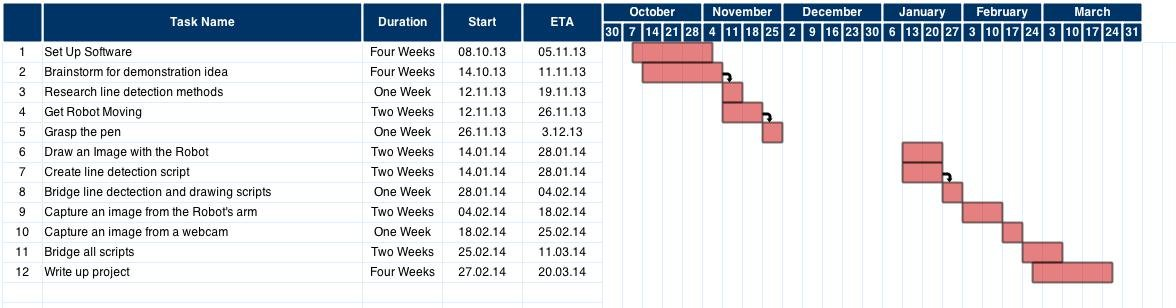
\includegraphics[width = 20cm, height = 6cm, angle=90]{TP3_Gantt}
\end{center}

\clearpage

\subsection{Pert Chart}
\label{sec:pert-chart}
\begin{center}
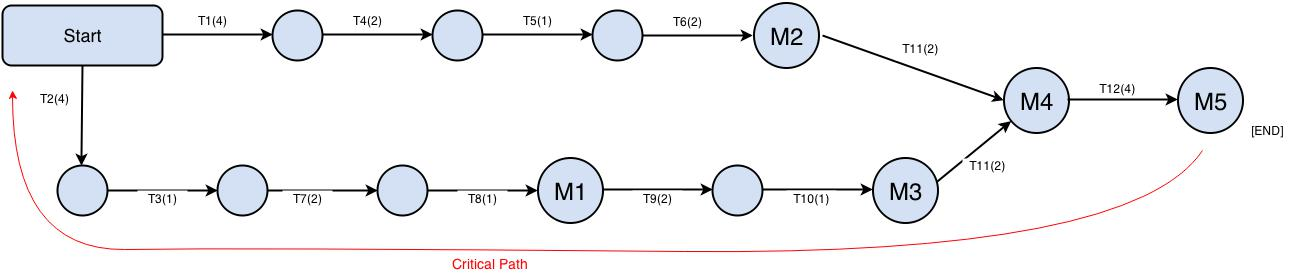
\includegraphics[width = 19cm, height = 6cm, angle=90]{TP3_PERT}
\end{center}
The task numbers relate to the same tasks and numbers from the above Gantt chart (section~\ref{sec:gantt-chart}, page~\pageref{sec:gantt-chart}).
\clearpage




\section{Implementation Design}
\subsection{Constraints}

\begin{tabular}{l p{12cm}}
\textbf {Speed} & The robot is only able to be run at a fraction of its total overall speed due to safety procedures in the case of an emergency stop.\\
\textbf {Cost} & The team have not been provided with funding for the project, so any demonstration will have to be within a very small budget.\\
\textbf {Isolation} & The robot is in a room of its own, and is viewed through perspex. Due to safety reasons nobody is allowed in the same room as the robot while the robot is running.\\
\textbf {Limited Movement} & The robot can only reach so far and it cannot rotate all 360 degrees on its axis, limiting its functionality.\\
\textbf {Weight restriction} & Despite weighing 750 kg, the robot's grippers are only strong enough to lift a maximum load of 2 kg. \\
\textbf {Dexterity} & As far as most robot’s go it is very dextrous but it still isn’t quite human.\\
\end{tabular}

\subsection{First Ideas}
Through brainstorming over our first three or four meetings we came up with a varying list of possible ideas for demonstrations. These demonstrations mainly inclued throwing various items, such as darts, bowling balls or pellets from a slingshot - which were all discarded as being unsuitable as each one breeched one of the constraints above. Finally, after several sessions we came up with an idea which would both (a) fulfil the constraints and (b) satisfy the requirements of the project.\\

\subsection{Final Design}
After several weeks of planning, we finally came up with our refined 'Artista' design. For this demonstration the robot will perform the following steps: 
\begin{itemize}
\item[--] capture an image of a participant from a webcam. See section~\ref{sec:imcap}, page~\pageref{sec:imcap} on Image Capturing for more information.
\item[--] perform a line detection algorithm on the image
\item[--] lift a pen placed on a tale in front of the robot
\item[--] draw the image of the participant's face
\end{itemize}
 
%+++++++++++++++++++++++++++++++++ANDY LOOK HERE :)+++++++++++++++++++++++++++++++++++++++++++++++++ 
 
\subsection{Design of Algorithms}
\textit{matlab pseudocode and diagram, improcessing.py pseudocode and diagram
 ANDY PLEASE COULD YOU WRITE THE PSEUDOCODE FOR THE IPAGEPROCESSING HERE, AND ALSO A DIAGRAM?}

\subsection{Design Evolution}
Thoughout a period of several weeks and throught the \textit{carrying out} of the projec the oriinal design evolved in a variety of ways. For example: 
\begin{itemize}
\item[--] \textit{The original design had the lid being removed by the other gripper}
\item[--] \textit{The original design had the other arm taking the picture through the glass}
\item[--] \textit{The original design had the other arm taking a birds eye capture of the finished drawing}
\end {itemize}
Through failure and experimentation (or through prototyping?) we discarded thses ideas from the original design due to complexity and time constraints. The logistics of removing the lid from the en with the other gripper and still maintain the correct drawing angle would be a very tough and time consuming script to produce. \\

%==============================================================================

\chapter{Implementation}
\section{Simulator}
The simulator we used for small scale testing came as part of the \acrshort{clopema} stack and is called RViz. Below is shown a figure of the UI of the RViz simulator program. (Figure ~\ref{fig:rviz}, page~\pageref{fig:rviz}).\\
RViz was extremely helpful at pointing out any potential flaws in our code before running it full scale, greatly reducing any safety concerns.\\
RViz was also advantageous as it allowed us to test our code more frequently, at times when we did not have access to the robot.

\begin{figure}[h!]
\centering
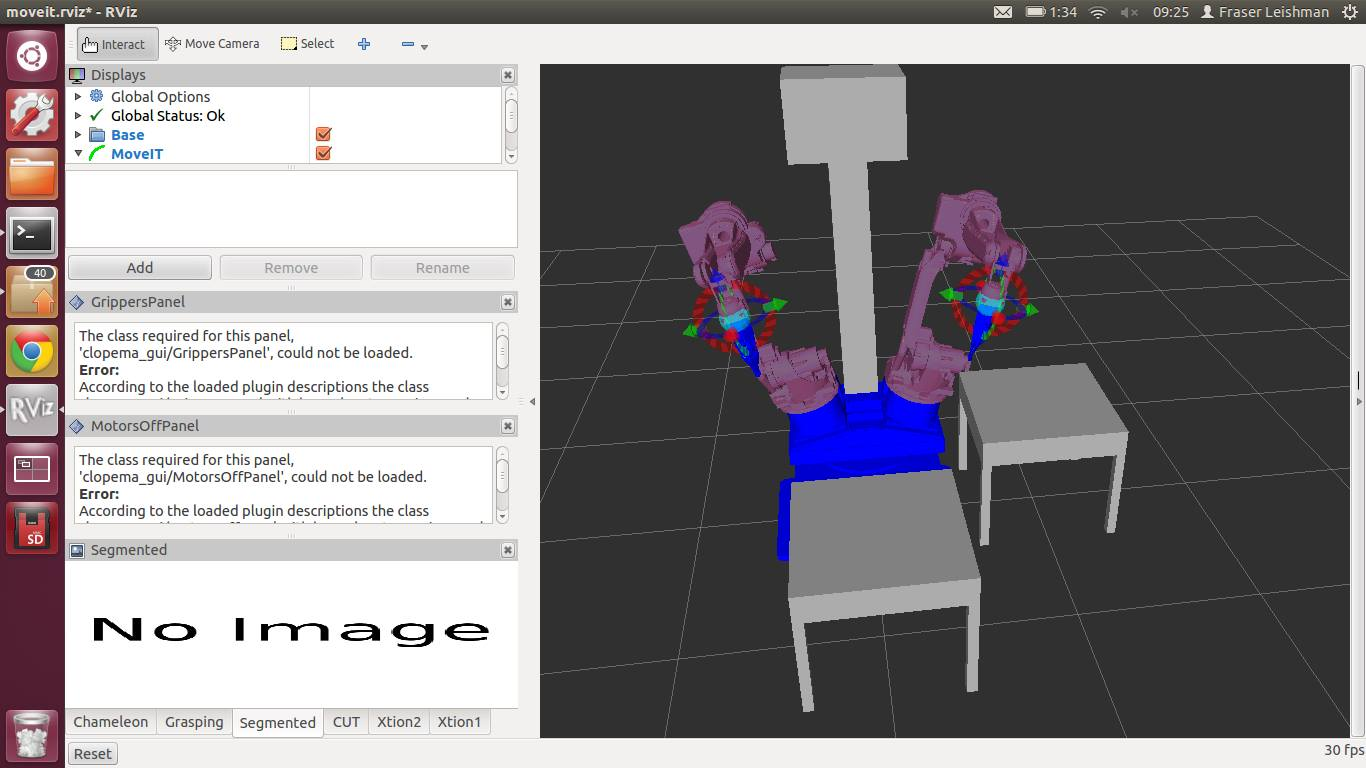
\includegraphics[width = 15cm, height = 8.36cm]{sim}
\caption{Screenshot of RViz simulator}
\label{fig:rviz}
\end{figure}

\pagebreak
\section{Image Capture}
\label{sec:imcap}
\subsection{Xtion}
The team were eager to use either \gls{xtion} to improve the overall functionality and "artistic talent" of the robot and so, we arrived at the idea of having one arm extend towards the participant in the observation room, take an image from the camera and them display it on the connected computer so that the taken image could be viewed before progressing on with the demonstration. The initial concern was that the perspex window would cause too much of a reflection and so spoil the taken image. Sadly, this was the case and a proposed solution was to have the particpant stand in a safe-spot inside the room that houses the robot and have the image taken from within and would result in no reflection.

This plan was well recieved by the team, but due to safety concerns that came along with having a student or anyone else in the room while the robot was active, the supervisor deemed this plan unsafe and so we had to come up with yet another solution.

\subsection{Webcam}
To combat this new problem, our new solution was to use a simple webcam that was mounted on top of a computer inside the robot's control room. This would negate any safety concerns and as there was no physical barrier between the camera and the participant, no reflections would be observed. A joint decision to implement the face detection that would have been present in the robot's camera was kept and therefore the webcam would be able to track the participants face whilst they were facing the camera through the use of the opensource \gls{opencv}. Finally, a face detected image would be cropped so that only the face was captured and all unnecessary background features would be removed. Once the initial process was complete, the image will be sent to the line detection script before it will be sent to the robot to start to draw. 

\section{Line Detection}
In order to detect lines on the image we used \gls{matlab}. This allowed us to write our own script which meant we could get each detail perfect. As the camera would always be stationary in the same spot with the same lighting conditions, \gls{matlab} allowed us to fine tune each value through experimentation in order to obtain an accurate line detection.
Another advantage of using \gls{matlab}, was that it also supported easy integration with python scripts used to drive the robot, using \gls{pymatbridge} - later discussed in section (~\ref{sec:pymatbridge}, page~\pageref{sec:pymatbridge})

\subsection{Background Noise}
After a variety of test images had been captured and processed, we noticed that there were extraneous lines that our image processing script had picked out as lines. These extra lines would appear in all of our initial photos and were finally deduced to be the background features of the image that were also present in each photo. By having each extra line, the overall completion time of the drawing would be increased and so, to maximise the efficiency of the program a couple of solutions were thought out.
\begin{itemize}
\item[--] {Only the face detected image would be captured so immediately any surrounding features would be cropped out as discussed in the previous section.}
\item[--] {Through the use of a green screen or similar item. By having a screen behind the participant any other features that could be been present in the ,now cropped, picture would be totally eliminated. This would result in a crisp as could be photo , ready to be converted.}
\end {itemize}
\section{Drawing Sketches}

\subsection{First Attempts}
For familiarise ourselves with the robot and its function, our first task was get the "hello world" equivalent of a robot. This would involve moving both of the arms upwards and then "wave" towards the users in the control room. This was thankfully quite straight forward for the team to accomplish.

The next task was to choose a predetermined position and place a marker pen, cap down, on the table.\\
As it was not viable to have the robot hold the pen in one hand and remove the cap with the other, the pen had to be carefully set up so that when the robot would attempt to grasp the pen, the cap would not be lifted up along with the body of the pen.\\
Due to this, when running our tests, every so often, both the cap and the pen would be grasped by the robot, forcing us to reset everything before we could begin again. While this is not the most practical method it was however, the easiest solution we could think of.

With the basic grasping completed, the next task we set ourselves was to draw a basic shape. A square is the easiest shape to draw as all that is required is four co-ordinates, each representing a corner. Four points were chosen and we set the robot up to draw. At first we deemed the test a success as what we could see was a drawn square. Instead, the drawing was actually curved which actually stumped the team as we could not think of a reasonable explination as to why the line would be curved. Eventually the cause of the curves were determined and it happened to be the algorithm that controlled the joints of the robot and which would pick the appropriate path to get between two points. Having this problem was out of ability as to fix something like that would require a complete overhaul of the current algorithm used by the robot. Instead of having a big square, we chose co-ordinates that were much closer together. Thankfully the reduced distance between corners would mean that the robot would draw straight lines.\\
For the final drawing though, we would need to be careful not to have any long lines as there would be no way to correct them.

\subsection{Curves}
Even though we had an issue with curved lines when trying to draw a straight line, a much greater problem was trying to intentionally draw curved lines. 
\subsection{Final Image}
\textit{drawing of the line dect image}
\section{Creating the Final Product}
\subsection{pymatbridge}
\label{sec:pymatbridge}
We used \gls{pymatbridge} to like the python scripts written to drive the robot and the \gls{matlab} script we had written to detect the lines on the image of the participant's face. 


%==============================================================================
\chapter{Evaluation}

\section{Evaluation}
\subsection{Methodology}

\subsection{High Level Goals}
The aim of the evaluation is to establish whether or not the implementation of a robotic artist was an exciting demonstration to show off the robots capabilities and also if the completed drawings would be considered artistic. We hope to discuss both the success the team achieved and also the flaws that were uncovered throughout development which will let us make future improvements.

\section{Future Work}
\subsection{Increasing Efficiency}
The main drawback that was found when drawing the detected face was the speed as to successfully draw the face took a running time of just over an hour. With this large time, it would be much more feasible if we could shave a large chunk of time off.Due to safety reasons the robot only runs at a small percentage of its maximum speed and is therefore quite slow. Knowing that this is a problem, any major improvement would be in choosing a more efficient method that would be used to create our vector image.


so any code should be as efficient as possible in order to prevent lengthening the demonstration any further. We feel that our algorithms could be made slightly more efficient, or even parallelised in order to increase this efficiency to slicken the deminstration.
If we were able to significantly improve the algorithms so that the demonstration was running quickly, we could perhaps look into using higher resolution images in order to make the drawings more recognisable.

\subsection{Recognising The Pen}
A far fetched plan would be to have the \gls{xtion} camera that are attached to the robot to first recognise the pen that is randomly placed on the table and then grasp it. This would be a very advanced feature to implement owing to the complexity of implementation. Furthermore, object recognition software would have to be used and then integrated with ROS which is way out of the teams current comfort zone. In the future, once the team have a greater grasp on ROS and othe componants then this may be a feature.

\subsection{Take Lid Off Pen}
What was once an initial idea, was scrapped early one. The robot would grasp the marker pen with one of it's arms and then the other would move and grasp the cap of the pen to pull it off. While this seems to be a realtively simple task this was actually deemed to be too ambitious for us to attempt. One of the possible reasons could be the risk of any collisions between arms as there is an exceptionally small margin of error when trying to move each arm close together. In future iterations of development, the team would like to add this as a feature because we feel that it adds an overall more artistic feel rather than having a cap already off.


\subsection{Bird's Eye Video Stream}
One of the discarded ideas from the original design was for the robot to reach its other arm up to a birds eye position and capture an image of the final drawing to be displayed on screen. If this project was to be developed in future we could firstly implement this stage, then perhaps take it further by moving the arm to this position at the start of the drawing and streaming the birds eye viewing from the robot's perspective onto the screen of the participant.

\subsection{Artistic Flair}
To enhance the overall spectacle of the demonstration, the robot could have displayed much more artistic flair. This would have involved using more striking and refined pen movements to mimic those a human artist would use. However, in robotics, one of the biggest problems that is faced is trying recreate the fluidity of human movement. To try and rectify the solid, blocky movements that the robot currently uses would potentially require the team to look into the current algorithm that the robot uses to determine its movement. Sadly this is also beyond the knowledge of the team and more practise would need to be had before being attempting this feature

Furthermore,a few comedic ideas were presented. A beret could have been placed on the robot to symbolise a stereotypical French artist. This idea could have been furthered by providing the robot with a French accent. While these two ideas do not provide much in the way of useful features, this comedic value will heighten the enjoyment of the participans experience which is what the main goal of the project has been.



%  
%==============================================================================
\chapter{Conclusion}
The basic concept of creating an engaging and exciting task for the \acrshort{clopema} robot to perform has been taken from the initial brainstorming of ideas to a fully functional artistic robot in a little over five months.Throughout the durtation of this project, the team worked very closely with a variety of open source programs that would help turn our ideas into a reality. 

Trying to learn and understand ROS was the most difficult process that was encountered. The initial lack of any knowledge regarding the basics of ROS was a massive hindrance which set the team back right from the get go. However, as time progressed each member became quite familiar with the software and in the latter stages of the project any changes made to the source code that would help the robot function could be implemented relatively easily. 

Working with \acrshort{clopema} robot itself was a very interesting experience for the whole team as none of the members had any prior experience in robotics and so, with our first interaction with it, there was a sense of nervousness and excitement among the team as we were excited to have a great opportunity to work with a high-calibre robot.

The robot was transformed from its initial function of folding and manipulating clothes to detecting faces and then drawing the face that was captured. This was a rather challanging prospect as the robot would seem to be so far out of its depth due to the complete change in function that would be required of it. However, due to careful planning we managed to successfully have the robot function as an artist.

Due to the limitations that were in place, in regards to the robot, we had to be as efficient as possible in order to maximise the potential of having a recognisable drawing completed. This is where our choice of open-source software came in. With OpenCV our efforts in trying to detect faces was greatly reduced due to the massive support that OpenCV boasts in respect to the vast multitude of libraries that are available for anyone to download and use freely. The other open-source software ROS was critical in maintaining efficiency as the basic commands of controlling the robot became much more understandable. This was only possible after a good understanding of ROS had been achieved.

Overall, the project presented us with a great opportunity to leap into the world of robotics which is something that very few, if any, undergradutate students are able to do. Working along side a researcher who is a member of the \acrshort{clopema} project was insightful in learning to understand how the word of robotics function.

As a team we worked very hard to overcome the hurdles that were highlighted thoughout this report and finally we can say that we achived what we aimed out to do, create an exciting and engaging demonstration to show off a robots capabilities.

%gobshite

\clearpage
\begin{appendices}
\chapter{Source Code Listing}
\section{FaceCrop.py}
\lstinputlisting[language=Python, breaklines=true]{faceCrop.py}
\newpage
\section{lineDect.m}
\lstinputlisting[language=Matlab, breaklines=true]{lineDect.m}
\newpage
\section{lineDect.py}
\lstinputlisting[language=Python, breaklines=true]{lineDect.py}
\newpage
\section{paint.py}
\lstinputlisting[language=Python, breaklines=true]{paint.py}
\newpage
\section{ImageProcessing.py}
\lstinputlisting[language=Python, breaklines=true]{ImageProcessing.py}
\end{appendices}
%
%==============================================================================
% using simplified bibliography
%see here http://en.wikibooks.org/wiki/LaTeX/Bibliography_Management

\begin{thebibliography}{1}
\addcontentsline{toc}{chapter}{Bibliography} %% puts bib into contents page

    \bibitem{middleware} \texttt{http://www.cs.wustl.edu/~wds/library/papers/2002/aaai-ss02.pdf}
    \bibitem{ros-desc} \texttt{http://wiki.ros.org/ROS/Introduction}
    \bibitem{ros-tutorials} \texttt{http://wiki.ros.org/ROS/Tutorials}
    \bibitem{robot-page} \texttt{http://clopemaweb.felk.cvut.cz/the-robot/}
    \bibitem{opencv}\texttt{matt fill this in for open cv}
    \bibitem{siebert-notes}{J. P. Siebert "Computer Vision Methods and Applications" (2013)
    \bibitem{edge-detection} \texttt{http://www.m-hikari.com/ams/ams-password-2008/ams-password29-32-2008/nadernejadAMS29-32-2008.pdf}
}
\end{thebibliography}
\clearpage
\printglossaries %displays all items in the glossary on its own page (auto adds to contents)


\clearpage
\chapter*{Acknowledgements}
\addcontentsline{toc}{chapter}{Acknowledgements}
\section*{Paul Siebert -- Project Supervisor}
As well as being our project supervisor and helping us stick to all deadlines and hand in dates etc. Paul was incredibly helpful with ths project, especially when it came to line detecting on the image. Paul was always happy to help and gave us a large amount of guidance throughout this project.
\section*{Gerardo Aragon Camarasa -- Research Assistant}
Gerardo was fantastic help. Being one of the major contributors to the \acrshort{clopema} project, he is entirely in the know when it comes to the robot. He was very helpful with all issues no matter how small and always had time for us. The project wouldn't be completed without Gerardo.
\section*{Douglas McFarlane -- DCS Support}
Douglas helped the team gain access to a computer with sudo access running \gls{ubuntu} in which we could install \acrshort{ros} and the \acrshort{clopema} stack in order to work on the project whilst on the university campus, this was a great help to us as it allowed us to collaboratively work on this one machine.

\end{document}
